\chapter{Transformer Architectures and Efficiency}
\label{sec:specialized_architectures}

\section{Introduction}
While Multi-Layer Perceptrons offer a generic learning model over vector inputs, they do not inherently leverage any underlying structure of the data. For this report, the architecture of interest is the Transformer. Since its introduction, the Transformer’s ability to model long-range dependencies in parallel has made it the foundation of state-of-the-art sequence modeling. However, this expressive power comes at a severe computational cost. To effectively compress such a model, one cannot treat it as a generic sequence of matrices; rather, one must deeply understand its internal wiring, where its parameters are concentrated, and how data moves through its layers during execution.

The purpose of this chapter is to dissect the Transformer architecture specifically through the lens of computational cost and structural parameterization. The chapter begins by detailing the core building blocks of the network—namely, the Multi-Head Attention mechanism and the position-wise Feed-Forward Networks (FFNs). Special emphasis is placed on the matrix dimensions and structural design of these components, as they dictate the exact locations of the parameters that pruning algorithms will later target.

Building on these components, the chapter then examines the complete Encoder-Decoder architecture before shifting focus to the primary motivation for this report: the computational bottleneck. We analyze the quadratic scaling of self-attention and the massive memory footprints of dense weight matrices. Finally, the chapter introduces hardware-aware efficiency metrics, such as FLOPs, memory bandwidth, and latency.



%, which has become the dominant model for sequence modeling tasks, particularly in natural language processing, and is the target of the compression methods discussed in later chapters.

%\subsection{Convolutional Neural Networks (CNNs)}
%
%CNNs are feedforward networks optimized for grid-like data, such as images. They stack multiple modules, typically consisting of:
%
%\begin{figure}[htbp]
%    \centering
%    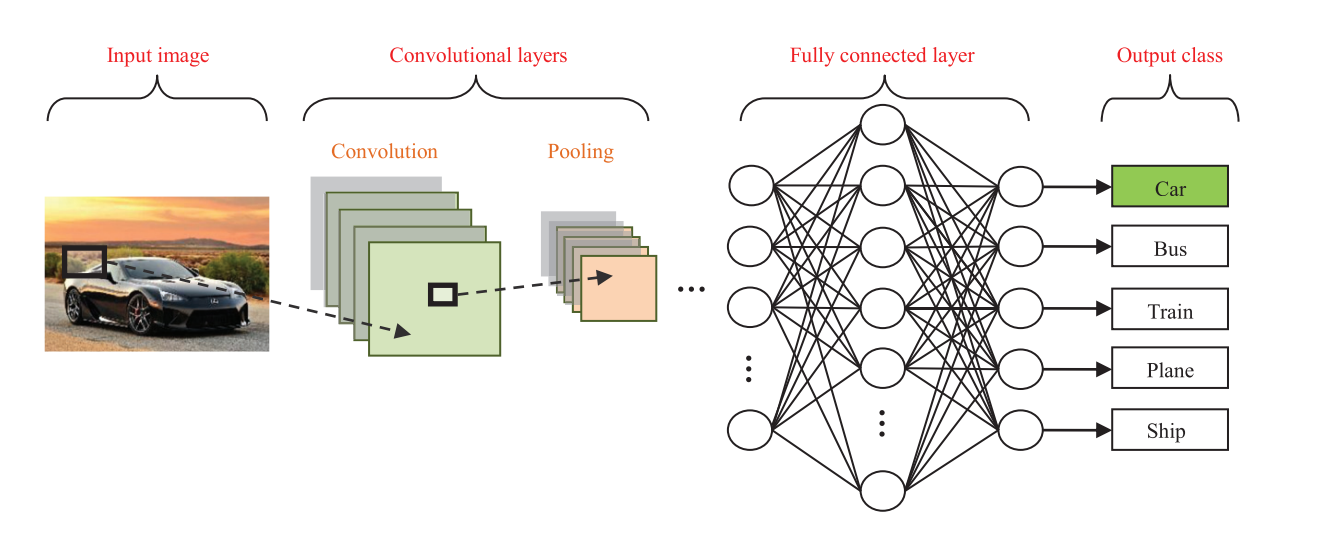
\includegraphics[width=0.85\textwidth]{figures/foundations/cnn_classification_pipeline}
%    \caption{Simple CNN architecture: input, convolution + activation, pooling, and fully connected layers \cite{Waseem2017}.}
%    \label{fig:cnn-simple}
%\end{figure}
%
%\begin{itemize}
%    \item \textbf{Convolutional Layers:} These act as feature extractors. A learnable filter (kernel) $K$ slides over the input $I$, performing element-wise multiplication and summation to create a feature map $S$. The operation is defined as:
%    \[
%    S(i, j) = (I * K)(i, j) = \sum_{m} \sum_{n} I(i+m, j+n) K(m, n)
%    \]
%    \item \textbf{Pooling Layers:} These reduce the spatial dimensions (width and height) of feature maps using summary statistics (e.g., Max or Average pooling) to decrease computational cost and overfitting.
%\end{itemize}
%
%\subsection{Recurrent Neural Networks (RNNs)}
%RNNs are designed for sequential data (e.g., time series, text). Unlike feedforward networks, RNNs utilize cyclic connections to maintain a \textit{hidden state} that captures historical information. The network dynamics are described by:
%\[
%h_t = \sigma(W_{hh} h_{t-1} + W_{xh} x_t + b_h)
%\]
%\[
%y_t = W_{hy} h_t + b_y
%\]
%where \( h_t \) is the hidden state, \( x_t \) the input, and \( y_t \) the output at time \( t \).
%\begin{figure}[htbp]
%  \centering
%  \begin{tikzpicture}[>=Stealth, node distance=10mm and 18mm, every node/.style={font=\small}]
%    \tikzstyle{inp} = [circle, draw=slateblue, fill=mistyblue!20, minimum size=7mm]
%    \tikzstyle{hid} = [rectangle, draw=dustyteal, fill=sagegreen!20, minimum size=9mm]
%    \tikzstyle{outnode} = [circle, draw=slateblue, fill=mistyblue!20, minimum size=7mm]
%    \tikzstyle{lbl} = [font=\scriptsize, color=slateblue]
%
%    % Inputs (bottom layer)
%    \node[inp] (x1) {$x_1$};
%    \node[inp] (x2) [right=of x1] {$x_2$};
%    \node[inp] (x3) [right=of x2] {$x_3$};
%    \node (xd) [right=of x3] {$\dots$};
%    \node[inp] (xT) [right=of xd] {$x_T$};
%
%    % Hidden (middle layer)
%    \node[hid] (h1) [above=of x1] {$h_1$};
%    \node[hid] (h2) [above=of x2] {$h_2$};
%    \node[hid] (h3) [above=of x3] {$h_3$};
%    \node[hid] (hT) [above=of xT] {$h_T$};
%    \node (hd) [right=of h3] {$\dots$};
%
%    % Outputs (top layer)
%    \node[outnode] (y1) [above=of h1] {$y_1$};
%    \node[outnode] (y2) [above=of h2] {$y_2$};
%    \node[outnode] (y3) [above=of h3] {$y_3$};
%    \node[outnode] (yT) [above=of hT] {$y_T$};
%
%    % Input to hidden
%    \draw[->] (x1) -- node[midway, left, lbl] {$W_{xh}$} (h1);
%    \draw[->] (x2) -- node[midway, left, lbl] {$W_{xh}$} (h2);
%    \draw[->] (x3) -- node[midway, left, lbl] {$W_{xh}$} (h3);
%    \draw[->] (xT) -- node[midway, left, lbl] {$W_{xh}$} (hT);
%
%    % Hidden recurrence
%    \draw[->] (h1) to[bend left=8] node[midway, above, lbl] {$W_{hh}$} (h2);
%    \draw[->] (h2) to[bend left=8] node[midway, above, lbl] {$W_{hh}$} (h3);
%    \draw[->] (h3) -- (hd);
%    \draw[->] (hd) to[bend left=8] node[midway, above, lbl] {$W_{hh}$} (hT);
%
%    % Hidden to Output
%    \draw[->] (h1) -- node[midway, left, lbl] {$W_{hy}$} (y1);
%    \draw[->] (h2) -- node[midway, left, lbl] {$W_{hy}$} (y2);
%    \draw[->] (h3) -- node[midway, left, lbl] {$W_{hy}$} (y3);
%    \draw[->] (hT) -- node[midway, left, lbl] {$W_{hy}$} (yT);
%
%    \node[below left=2mm and 6mm of h1, font=\scriptsize] (h0label) {$h_0$};
%    \draw[->] (h0label.north) to[bend left=20] (h1.west);
%  \end{tikzpicture}
%  \caption{RNN unrolled in time.}
%  \label{fig:rnn-compact}
%\end{figure}
%
%\subsection{Autoencoders (AEs)}
%
%Autoencoders are neural networks designed for unsupervised learning of efficient data codings. They act as an identity function that learns to compress and then reconstruct data. An AE consists of two main parts:
%
%\begin{figure}[htbp]
%    \centering
%    \begin{tikzpicture}[>=Stealth, node distance=15mm, every node/.style={font=\small}]
%
%        % Define styles matching your previous RNN colors
%        % If these colors are defined in your preamble, you can remove these \definecolor lines
%        \definecolor{slateblue}{RGB}{106,90,205}
%        \definecolor{mistyblue}{RGB}{224,238,238}
%        \definecolor{dustyteal}{RGB}{76,146,147}
%        \definecolor{sagegreen}{RGB}{193,225,193}
%
%        \tikzstyle{neuron} = [circle, draw=slateblue, fill=mistyblue!20, minimum size=7mm, inner sep=0pt]
%        \tikzstyle{bottleneck} = [circle, draw=dustyteal, fill=sagegreen!20, minimum size=7mm, inner sep=0pt]
%        \tikzstyle{lbl} = [font=\scriptsize, color=slateblue]
%
%        % --- Nodes ---
%
%        % Input Layer (x)
%        \node[neuron] (i1) at (0, 2.0) {};
%        \node[neuron] (i2) at (0, 1.0) {};
%        \node[neuron] (i3) at (0, 0.0) {};
%        \node[neuron] (i4) at (0, -1.0) {};
%        \node[neuron] (i5) at (0, -2.0) {};
%
%        % Encoder Hidden
%        \node[neuron] (e1) at (2, 1.2) {};
%        \node[neuron] (e2) at (2, 0) {};
%        \node[neuron] (e3) at (2, -1.2) {};
%
%        % Bottleneck / Latent Space (z)
%        \node[bottleneck] (z1) at (4, 0.5) {};
%        \node[bottleneck] (z2) at (4, -0.5) {};
%
%        % Decoder Hidden
%        \node[neuron] (d1) at (6, 1.2) {};
%        \node[neuron] (d2) at (6, 0) {};
%        \node[neuron] (d3) at (6, -1.2) {};
%
%        % Output Layer (x_hat)
%        \node[neuron] (o1) at (8, 2.0) {};
%        \node[neuron] (o2) at (8, 1.0) {};
%        \node[neuron] (o3) at (8, 0.0) {};
%        \node[neuron] (o4) at (8, -1.0) {};
%        \node[neuron] (o5) at (8, -2.0) {};
%
%        % --- Connections ---
%
%        % Input -> Encoder
%        \foreach \i in {1,...,5}
%            \foreach \j in {1,...,3}
%                \draw[->, slateblue!40] (i\i) -- (e\j);
%
%        % Encoder -> Bottleneck
%        \foreach \i in {1,...,3}
%            \foreach \j in {1,...,2}
%                \draw[->, slateblue!40] (e\i) -- (z\j);
%
%        % Bottleneck -> Decoder
%        \foreach \i in {1,...,2}
%            \foreach \j in {1,...,3}
%                \draw[->, slateblue!40] (z\i) -- (d\j);
%
%        % Decoder -> Output
%        \foreach \i in {1,...,3}
%            \foreach \j in {1,...,5}
%                \draw[->, slateblue!40] (d\i) -- (o\j);
%
%        % --- Labels ---
%
%        \node[below=0.2cm of i5] {Input $x$};
%        \node[below=0.2cm of o5] {Output $\hat{x}$};
%        \node[below=0.2cm of z2, align=center] {Latent\\Space $z$};
%
%        % Braces for Encoder/Decoder
%        \draw[decorate, decoration={brace, amplitude=10pt, raise=5pt}, thick, slateblue] (i1.north) -- (z1.north) node[midway, above=20pt] {\textbf{Encoder}};
%        \draw[decorate, decoration={brace, amplitude=10pt, raise=5pt}, thick, slateblue] (z1.north) -- (o1.north) node[midway, above=20pt] {\textbf{Decoder}};
%
%    \end{tikzpicture}
%    \caption{Autoencoder architecture: The input is compressed into a lower-dimensional latent space (Bottleneck) and then reconstructed.}
%    \label{fig:autoencoder}
%\end{figure}
%
%\begin{itemize}
%    \item \textbf{Encoder:} Maps the high-dimensional input $x$ to a lower-dimensional latent representation $z$.
%    \item \textbf{Decoder:} Reconstructs the output $\hat{x}$ from the latent representation $z$.
%\end{itemize}
%
%The network is trained to minimize the reconstruction error (e.g., Mean Squared Error) between the input and the output:
%\[
%L(x, \hat{x}) = || x - \hat{x} ||^2
%\]
%By forcing data through a bottleneck, the network learns to capture the most salient features of the data distribution.
%

\newpage
\section{Transformer Networks}

Transformer networks, introduced by \cite{vaswani2017attention}, changed sequence modeling by replacing recurrent processing with attention-based computation. Instead of processing tokens one after another, a Transformer can compare tokens across the whole sequence in parallel. This makes it highly effective for language modelling, translation, summarization, and other sequence tasks. The original architecture was an encoder-decoder model for machine translation, while later systems often use encoder-only variants such as BERT \cite{devlin2019bert} or decoder-only variants such as LLaMA \cite{touvron2023llama2}.

\section{Core Architectural Components: Building Blocks of the Transformer}

Before separating the model into encoder and decoder stacks, it is useful to define the components repeated inside those stacks. Transformer layers are built from token embeddings, positional information, attention projections, feed-forward channels, residual connections, and normalization layers. These components are also the main targets for compression, because they determine both parameter count and runtime cost.

\subsubsection{Input Representation: Embeddings and Positional Encoding}

Every token is mapped to a continuous embedding vector. Since self-attention does not inherently encode token order, positional information is added to the token representations. The original Transformer uses sinusoidal positional encodings \cite{vaswani2017attention}, shown in Eq.\eqref{eq:positional_encoding}, where $d_{\text{model}}$ is the embedding dimension and $i$ indexes the dimensions of the positional encoding:
\begin{equation}
  \label{eq:positional_encoding}
    PE_{(\text{pos}, 2i)} = \sin\left(\frac{\text{pos}}{10000^{2i/d_{\text{model}}}}\right), \quad
    PE_{(\text{pos}, 2i+1)} = \cos\left(\frac{\text{pos}}{10000^{2i/d_{\text{model}}}}\right).
\end{equation}

\subsubsection{Self-Attention Mechanism}

Self-attention allows each token representation to aggregate information from the rest of the sequence. The mechanism uses three learned projections of each input: queries, keys, and values \cite{vaswani2017attention}. Queries represent what a token is looking for, keys represent what each token offers for comparison, and values contain the information that will be aggregated.

For an input sequence representation $\matr{X} \in \reals^{n \times d_{\text{model}}}$, the projections are computed as shown in Eq.\eqref{eq:attention_projections}, where $\matr{W}^{Q}, \matr{W}^{K}, \matr{W}^{V} \in \reals^{d_{\text{model}} \times d_k}$ are learned weight matrices for queries, keys, and values respectively:
\begin{equation}
  \label{eq:attention_projections}
    \matr{Q} = \matr{X}\matr{W}^{Q}, \quad
    \matr{K} = \matr{X}\matr{W}^{K}, \quad
    \matr{V} = \matr{X}\matr{W}^{V}.
\end{equation}

Scaled dot-product attention is then computed as shown in Eq.\eqref{eq:scaled_dot_product_attention}, where $d_k$ is the dimension of the queries and keys:
\begin{equation}
  \label{eq:scaled_dot_product_attention}
    \operatorname{Attention}(\matr{Q}, \matr{K}, \matr{V})
    =
    \operatorname{softmax}\left(\frac{\matr{Q}\matr{K}^{\top}}{\sqrt{d_k}}\right)\matr{V}.
\end{equation}
The factor $\sqrt{d_k}$ prevents dot products from becoming too large, which would push the softmax into saturated regions with weak gradients.

\subsubsection{Multi-Head Attention}

Multi-head attention applies several attention mechanisms in parallel, allowing the model to attend to different representation subspaces and token relationships at the same time \cite{vaswani2017attention}. Eq.\eqref{eq:multi_head_attention} defines the computation for each head $i$, where $\matr{W}^{Q}_{i}, \matr{W}^{K}_{i}, \matr{W}^{V}_{i} \in \reals^{d_{\text{model}} \times d_k}$ are the projection matrices for head $i$:
\begin{equation}
  \label{eq:multi_head_attention}
    \operatorname{head}_i =
    \operatorname{Attention}(\matr{X}\matr{W}^{Q}_{i}, \matr{X}\matr{W}^{K}_{i}, \matr{X}\matr{W}^{V}_{i}),
    \quad i = 1,\ldots,h.
\end{equation}

The head outputs are concatenated and projected back to the model dimension as expressed in Eq.\eqref{eq:multi_head_concat_projection}, where $\matr{W}^{O} \in \reals^{hd_v \times d_{\text{model}}}$ is the output projection matrix:
\begin{equation}
  \label{eq:multi_head_concat_projection}
    \operatorname{MultiHead}(\matr{X}) =
    \operatorname{Concat}(\operatorname{head}_1,\ldots,\operatorname{head}_h)\matr{W}^{O}.
\end{equation}
\subsubsection{Feed-Forward Network}

After attention mixes information across tokens, a position-wise Feed-Forward Network (FFN) processes each token representation independently
The FFN usually expands the hidden representation to a larger intermediate dimension $d_{ff}$ and then projects it back to $d_{\text{model}}$. In the original Transformer, $d_{ff}$ is typically much larger than $d_{\text{model}}$, making FFN channels a major source of parameters and a natural target for structured pruning.

\subsubsection{Residual Connections and Layer Normalization}

Each attention or FFN sub-layer is wrapped by a residual path and layer normalization. Residual connections preserve a direct path for information and gradients, while normalization stabilizes the scale of hidden representations. This design is essential for training deep Transformer stacks and is also important when later compression methods remove heads, channels, or blocks \cite{vaswani2017attention,He2016,Ba2016}.

\subsection{Encoder and Decoder Architecture}

With the core components defined, the encoder and decoder can be described cleanly. The full encoder-decoder Transformer contains two main stacks:
\begin{itemize}
    \item \textbf{Encoder:} Processes the complete input sequence in parallel and produces contextual source representations.
    \item \textbf{Decoder:} Generates the output sequence autoregressively while attending to both previous target tokens and the encoder output.
\end{itemize}

The encoder converts the source sequence into a contextual memory representation $\matr{H}_{\text{enc}}$. The decoder uses this memory through cross-attention while also using masked self-attention to prevent access to future target tokens. The complete architecture is shown in Figure~\ref{fig:transformer-architecture}.

\begin{figure}[H]
  \centering
  \begin{tikzpicture}[scale=1.2, transform shape]
    \tikzstyle{Sanode} = [minimum height=1.4em, minimum width=7em, inner sep=3pt, rounded corners=1.5pt, draw=slateblue, fill=mistyblue!30]
    \tikzstyle{Resnode} = [minimum height=1.1em, minimum width=7em, inner sep=3pt, rounded corners=1.5pt, draw=dustyteal, fill=softgray!30]
    \tikzstyle{ffnnode} = [minimum height=1.4em, minimum width=7em, inner sep=3pt, rounded corners=1.5pt, draw=slateblue, fill=sagegreen!30]
    \tikzstyle{outputnode} = [minimum height=1.4em, minimum width=7em, inner sep=3pt, rounded corners=1.5pt, draw=slateblue, fill=mistyblue!50]
    \tikzstyle{inputnode} = [minimum height=1.4em, minimum width=3.5em, inner sep=3pt, rounded corners=1.5pt, draw=dustyteal, fill=mistyblue!20]
    \tikzstyle{posnode} = [minimum height=1.4em, minimum width=3.5em, inner sep=3pt, rounded corners=1.5pt, draw=dustyteal, fill=softgray!50]
    \tikzstyle{standard} = [rounded corners=3pt]

    \node [Sanode, anchor=west] (sa1) at (0,0) {\tiny \textbf{Self-Attention}};
    \node [Resnode, anchor=south] (res1) at ([yshift=0.3em]sa1.north) {\tiny \textbf{Add \& LayerNorm}};
    \node [ffnnode, anchor=south] (ffn1) at ([yshift=1em]res1.north) {\tiny \textbf{FFN}};
    \node [Resnode, anchor=south] (res2) at ([yshift=0.3em]ffn1.north) {\tiny \textbf{Add \& LayerNorm}};
    \node [inputnode, anchor=north west] (input1) at ([yshift=-1em,xshift=-0.5em]sa1.south west) {\tiny \textbf{Emb.}};
    \node [] (add1) at ([yshift=-1.6em,xshift=3.5em]sa1.south west) {$+$};
    \node [posnode, anchor=north east] (pos1) at ([yshift=-1em,xshift=0.5em]sa1.south east) {\tiny \textbf{Position}};
    \node [anchor=south] (encoder) at ([xshift=0.2em,yshift=0.6em]res2.north west) {\scriptsize \textbf{Encoder}};
    \draw [->,dustyteal] ([yshift=-4em]sa1.south) -- (add1);

    \draw [->,dustyteal] (sa1.north) -- (res1.south);
    \draw [->,dustyteal] (res1.north) -- (ffn1.south);
    \draw [->,dustyteal] (ffn1.north) -- (res2.south);
    \draw [->,dustyteal] ([yshift=-1em]sa1.south) -- (sa1.south);

    \node [Sanode, anchor=west] (sa2) at ([xshift=3em]sa1.east) {\tiny \textbf{Masked Self-Attn}};
    \node [Resnode, anchor=south] (res3) at ([yshift=0.3em]sa2.north) {\tiny \textbf{Add \& LayerNorm}};
    \node [Sanode, anchor=south] (ed1) at ([yshift=1em]res3.north) {\tiny \textbf{Cross-Attention}};
    \node [Resnode, anchor=south] (res4) at ([yshift=0.3em]ed1.north) {\tiny \textbf{Add \& LayerNorm}};
    \node [ffnnode, anchor=south] (ffn2) at ([yshift=1em]res4.north) {\tiny \textbf{FFN}};
    \node [Resnode, anchor=south] (res5) at ([yshift=0.3em]ffn2.north) {\tiny \textbf{Add \& LayerNorm}};
    \node [outputnode, anchor=south] (o1) at ([yshift=1em]res5.north) {\tiny \textbf{Linear + Softmax}};
    \node [inputnode, anchor=north west] (input2) at ([yshift=-1em,xshift=-0.5em]sa2.south west) {\tiny \textbf{Emb.}};
    \node [] (add) at ([yshift=-1.6em,xshift=3.5em]sa2.south west) {$+$};
    \node [posnode, anchor=north east] (pos2) at ([yshift=-1em,xshift=0.5em]sa2.south east) {\tiny \textbf{Position}};
    \node [anchor=east] (decoder) at ([xshift=-1em,yshift=-1.5em]o1.west) {\scriptsize \textbf{Decoder}};

    \draw[<-, dustyteal] (add.south) -- ++(0,-1.5em);

    \draw [->,dustyteal] (sa2.north) -- (res3.south);
    \draw [->,dustyteal] (res3.north) -- (ed1.south);
    \draw [->,dustyteal] (ed1.north) -- (res4.south);
    \draw [->,dustyteal] (res4.north) -- (ffn2.south);
    \draw [->,dustyteal] (ffn2.north) -- (res5.south);
    \draw [->,dustyteal] (res5.north) -- (o1.south);
    \draw [->,dustyteal] (o1.north) -- ([yshift=0.5em]o1.north);
    \draw [->,dustyteal] ([yshift=-1em]sa2.south) -- (sa2.south);

    \draw[->,standard,dustyteal] ([yshift=-0.5em]sa1.south) -- ([xshift=-4em,yshift=-0.5em]sa1.south) -- ([xshift=-4em,yshift=2.3em]sa1.south) -- ([xshift=-3.5em,yshift=2.3em]sa1.south);
    \draw[->,standard,dustyteal] ([yshift=0.5em]res1.north) -- ([xshift=-4em,yshift=0.5em]res1.north) -- ([xshift=-4em,yshift=3.3em]res1.north) -- ([xshift=-3.5em,yshift=3.3em]res1.north);
    \draw[->,standard,dustyteal] ([yshift=-0.5em]sa2.south) -- ([xshift=4em,yshift=-0.5em]sa2.south) -- ([xshift=4em,yshift=2.3em]sa2.south) -- ([xshift=3.5em,yshift=2.3em]sa2.south);
    \draw[->,standard,dustyteal] ([yshift=0.5em]res3.north) -- ([xshift=4em,yshift=0.5em]res3.north) -- ([xshift=4em,yshift=3.3em]res3.north) -- ([xshift=3.5em,yshift=3.3em]res3.north);
    \draw[->,standard,dustyteal] ([yshift=0.5em]res4.north) -- ([xshift=4em,yshift=0.5em]res4.north) -- ([xshift=4em,yshift=3.3em]res4.north) -- ([xshift=3.5em,yshift=3.3em]res4.north);
    \draw[->,standard, line width=1.2pt, slateblue] (res2.north) -- ([yshift=0.5em]res2.north) -- ([xshift=5em,yshift=0.5em]res2.north) -- ([xshift=5em,yshift=-2.2em]res2.north) -- ([xshift=6.5em,yshift=-2.2em]res2.north);
    \node[font=\tiny, slateblue] at ([xshift=5.5em,yshift=-1.5em]res2.north) {$\matr{H}_{\text{enc}}$};

  \end{tikzpicture}
  \caption{Complete Encoder-Decoder Transformer architecture}
  \label{fig:transformer-architecture}
\end{figure}

\subsubsection{The Encoder Stack}

An encoder layer contains multi-head self-attention followed by a feed-forward network, with residual connections and normalization around each sub-layer. In encoder self-attention, the queries, keys, and values all come from the same source sequence. This makes the encoder bidirectional: every input token can attend to every other input token. Figure~\ref{fig:encoder} shows the internal order of these operations before the resulting representation is passed to the decoder. After $N$ encoder layers, the output is the memory matrix $\matr{H}_{\text{enc}} \in \reals^{n \times d_{\text{model}}}$, which summarizes the source sequence for the decoder.

\begin{figure}[H]
  \centering
  \begin{tikzpicture}[scale=1.0, transform shape]
    \tikzstyle{Sanode} = [minimum height=1.4em, minimum width=7em, inner sep=3pt, rounded corners=1.5pt, draw=slateblue, fill=mistyblue!30]
    \tikzstyle{Resnode} = [minimum height=1.1em, minimum width=7em, inner sep=3pt, rounded corners=1.5pt, draw=dustyteal, fill=softgray!30]
    \tikzstyle{ffnnode} = [minimum height=1.4em, minimum width=7em, inner sep=3pt, rounded corners=1.5pt, draw=slateblue, fill=sagegreen!30]
    \tikzstyle{inputnode} = [minimum height=1.4em, minimum width=3.5em, inner sep=3pt, rounded corners=1.5pt, draw=dustyteal, fill=mistyblue!20]
    \tikzstyle{posnode} = [minimum height=1.4em, minimum width=3.5em, inner sep=3pt, rounded corners=1.5pt, draw=dustyteal, fill=softgray!50]
    \tikzstyle{standard} = [rounded corners=3pt]

    \node [Sanode, anchor=west] (sa1) at (0,0) {\tiny \textbf{Self-Attention}};
    \node [Resnode, anchor=south] (res1) at ([yshift=0.3em]sa1.north) {\tiny \textbf{Add \& LayerNorm}};
    \node [ffnnode, anchor=south] (ffn1) at ([yshift=1em]res1.north) {\tiny \textbf{FFN}};
    \node [Resnode, anchor=south] (res2) at ([yshift=0.3em]ffn1.north) {\tiny \textbf{Add \& LayerNorm}};
    \node [inputnode, anchor=north west] (input1) at ([yshift=-1em,xshift=-0.5em]sa1.south west) {\tiny \textbf{Emb.}};
    \node [] (add1) at ([yshift=-1.6em,xshift=3.5em]sa1.south west) {$+$};
    \node [posnode, anchor=north east] (pos1) at ([yshift=-1em,xshift=0.5em]sa1.south east) {\tiny \textbf{Position}};


    \draw[<-, dustyteal] (add1.south) -- ++(0,-1.5em);

    \draw [->,dustyteal] (sa1.north) -- (res1.south);
    \draw [->,dustyteal] (res1.north) -- (ffn1.south);
    \draw [->,dustyteal] (ffn1.north) -- (res2.south);
    \draw [->,dustyteal] ([yshift=-1em]sa1.south) -- (sa1.south);

    \draw[->,standard,dustyteal] ([yshift=-0.5em]sa1.south) -- ([xshift=-4em,yshift=-0.5em]sa1.south) -- ([xshift=-4em,yshift=2.3em]sa1.south) -- ([xshift=-3.5em,yshift=2.3em]sa1.south);
    \draw[->,standard,dustyteal] ([yshift=0.5em]res1.north) -- ([xshift=-4em,yshift=0.5em]res1.north) -- ([xshift=-4em,yshift=3.3em]res1.north) -- ([xshift=-3.5em,yshift=3.3em]res1.north);

  \end{tikzpicture}
  \caption{Transformer encoder layer architecture}
  \label{fig:encoder}
\end{figure}

\subsubsection{The Decoder Stack}

A decoder layer adds masked self-attention and cross-attention before the feed-forward network, enabling autoregressive generation while attending to encoder outputs. Masked self-attention restricts token $t$ to positions $\leq t$, preventing information leakage from future target tokens. Cross-attention then links the decoder to the encoder: decoder states act as queries, while encoder states provide keys and values. Figure~\ref{fig:decoder} shows this additional cross-attention block, which is the main structural difference between the decoder layer and the encoder layer.

\begin{figure}[H]
  \centering
  \begin{tikzpicture}[scale=1.0, transform shape]
    \tikzstyle{Sanode} = [minimum height=1.4em, minimum width=7em, inner sep=3pt, rounded corners=1.5pt, draw=slateblue, fill=mistyblue!30]
    \tikzstyle{Resnode} = [minimum height=1.1em, minimum width=7em, inner sep=3pt, rounded corners=1.5pt, draw=dustyteal, fill=softgray!30]
    \tikzstyle{ffnnode} = [minimum height=1.4em, minimum width=7em, inner sep=3pt, rounded corners=1.5pt, draw=slateblue, fill=sagegreen!30]
    \tikzstyle{outputnode} = [minimum height=1.4em, minimum width=7em, inner sep=3pt, rounded corners=1.5pt, draw=slateblue, fill=mistyblue!50]
    \tikzstyle{inputnode} = [minimum height=1.4em, minimum width=3.5em, inner sep=3pt, rounded corners=1.5pt, draw=dustyteal, fill=mistyblue!20]
    \tikzstyle{posnode} = [minimum height=1.4em, minimum width=3.5em, inner sep=3pt, rounded corners=1.5pt, draw=dustyteal, fill=softgray!50]
    \tikzstyle{standard} = [rounded corners=3pt]

    \node [Sanode, anchor=west] (sa2) at (0,0) {\tiny \textbf{Masked Self-Attn}};
    \node [Resnode, anchor=south] (res3) at ([yshift=0.3em]sa2.north) {\tiny \textbf{Add \& LayerNorm}};
    \node [Sanode, anchor=south] (ed1) at ([yshift=1em]res3.north) {\tiny \textbf{Cross-Attention}};
    \node [Resnode, anchor=south] (res4) at ([yshift=0.3em]ed1.north) {\tiny \textbf{Add \& LayerNorm}};
    \node [ffnnode, anchor=south] (ffn2) at ([yshift=1em]res4.north) {\tiny \textbf{FFN}};
    \node [Resnode, anchor=south] (res5) at ([yshift=0.3em]ffn2.north) {\tiny \textbf{Add \& LayerNorm}};
    \node [outputnode, anchor=south] (o1) at ([yshift=1em]res5.north) {\tiny \textbf{Linear + Softmax}};
    \node [inputnode, anchor=north west] (input2) at ([yshift=-1em,xshift=-0.5em]sa2.south west) {\tiny \textbf{Emb.}};
    \node [] (add) at ([yshift=-1.6em,xshift=3.5em]sa2.south west) {$+$};
    \node [posnode, anchor=north east] (pos2) at ([yshift=-1em,xshift=0.5em]sa2.south east) {\tiny \textbf{Position}};
    \node [anchor=south] (decoder) at ([xshift=0.2em,yshift=0.6em]o1.north west) {\scriptsize \textbf{Decoder}};

    \draw [->,dustyteal] ([yshift=-4em]sa2.south) -- (add);

    \draw [->,dustyteal] (sa2.north) -- (res3.south);
    \draw [->,dustyteal] (res3.north) -- (ed1.south);
    \draw [->,dustyteal] (ed1.north) -- (res4.south);
    \draw [->,dustyteal] (res4.north) -- (ffn2.south);
    \draw [->,dustyteal] (ffn2.north) -- (res5.south);
    \draw [->,dustyteal] (res5.north) -- (o1.south);
    \draw [->,dustyteal] (o1.north) -- ([yshift=0.5em]o1.north);
    \draw [->,dustyteal] ([yshift=-1em]sa2.south) -- (sa2.south);

    \draw[->,standard,dustyteal] ([yshift=-0.5em]sa2.south) -- ([xshift=4em,yshift=-0.5em]sa2.south) -- ([xshift=4em,yshift=2.3em]sa2.south) -- ([xshift=3.5em,yshift=2.3em]sa2.south);
    \draw[->,standard,dustyteal] ([yshift=0.5em]res3.north) -- ([xshift=4em,yshift=0.5em]res3.north) -- ([xshift=4em,yshift=3.3em]res3.north) -- ([xshift=3.5em,yshift=3.3em]res3.north);
    \draw[->,standard,dustyteal] ([yshift=0.5em]res4.north) -- ([xshift=4em,yshift=0.5em]res4.north) -- ([xshift=4em,yshift=3.3em]res4.north) -- ([xshift=3.5em,yshift=3.3em]res4.north);

  \end{tikzpicture}
  \caption{Transformer decoder layer architecture}
  \label{fig:decoder}
\end{figure}

\subsubsection{Encoder-Decoder Information Flow}

The complete sequence-to-sequence computation proceeds as follows:
\begin{enumerate}[leftmargin=*]
  \item \textbf{Encoding phase.} Source tokens $\vect{x}=(x_1,\ldots,x_n)$ are embedded, combined with positional information, and passed through $N$ encoder layers. The output is $\matr{H}_{\text{enc}}$.
  \item \textbf{Decoding phase.} Target tokens $\vect{y}=(y_1,\ldots,y_t)$ are embedded and processed autoregressively. Each decoder layer applies masked self-attention, cross-attention over $\matr{H}_{\text{enc}}$, and a feed-forward transformation.
  \item \textbf{Output phase.} The final decoder representation is projected to vocabulary logits. A softmax layer converts logits into token probabilities, and the selected token is fed back into the decoder at the next step.
\end{enumerate}



At this point in the report, we can view the Transformer as an arrangement of embedding layers, attention layers, feed-forward functions, and encoder--decoder connections. This architecture accounts for why it performs well on sequence modelling tasks, since each position can refine its representation using information from the rest of the sequence. This expressive structure, however, is computationally demanding. The next point examines where this cost arises inside the Transformer architecture.

\subsection{The Computational Bottleneck of Transformers}
\label{sec:transformer_bottleneck}
While powerful, the Transformer's success comes at a significant computational cost, which forms a central motivation for the compression techniques explored in this report. The standard Transformer architecture replaces recurrence with self-attention, enabling strong parallelism and high performance across sequence modelling tasks~\cite{vaswani2017attention}. However, this advantage comes with a major bottleneck: in full self-attention, each token attends to every other token in the sequence. For a sequence of length $n$, this requires an attention score matrix of size $n \times n$, making the attention component scale quadratically with sequence length in both computation and memory~\cite{beltagy2020longformer,tay2020efficient}.

This quadratic behaviour has direct practical implications. Doubling the sequence length from $512$ to $1024$ multiplies the attention matrix size by four, since $1024^2 / 512^2 = 4$. As a result, processing long documents or long-context inputs becomes substantially more expensive, which has motivated a large body of work on efficient Transformer variants and sparse or linear attention mechanisms~\cite{beltagy2020longformer,tay2020efficient}.

At the same time, modern language models benefit strongly from scaling model size, training data, and compute~\cite{kaplan2020scaling}. Later scaling-law work further showed that model size and the number of training tokens should be scaled together under a fixed compute budget, highlighting the continuing importance of large-scale training~\cite{hoffmann2022training}. This creates a tension between scale and deployment: larger models often achieve better performance, but practical inference is constrained by latency, memory, energy, and hardware availability. This tension motivates compression methods such as pruning, quantization, and knowledge distillation~\cite{han2015deep,sanh2019distilbert}.



The computational bottleneck defined above can be considered in several different ways. A Transformer may be expensive because of the size of its parameters, the memory required for activations, the number of arithmetic operations it performs, or the time required to run it on a specific hardware platform. Before discussing model efficiency in more detail, it is therefore useful to introduce the most common measures used to assess computational cost.
